\documentclass{standalone}
\usepackage{fontspec}
\usepackage{tikz}
\usetikzlibrary{arrows.meta,calc,positioning}
\begin{document}
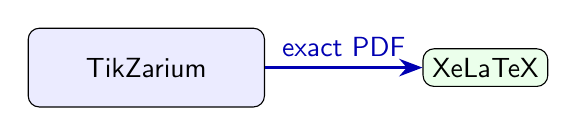
\begin{tikzpicture}[>=Stealth, every node/.style={font=\sffamily}]
  \node[draw,rounded corners,fill=blue!8,minimum width=3cm,minimum height=1cm] (A) {TikZarium};
  \node[draw,rounded corners,fill=green!8,right=2cm of A] (B) {XeLaTeX};
  \draw[->,very thick,blue!70!black] (A) -- node[above] {exact PDF} (B);
\end{tikzpicture}
\end{document}
